\documentclass[12pt, fleqn]{article}
\usepackage{../../../template/template}

%сам документ
\begin{document}
\begin{center}
  \huge Практика по дифференциальным уравнениям, 3 сем

  \Large (преподаватель Звягинцева Т. Е.)

  \large Записал Костин П.А.
\end{center}

Данный документ неидеальный, прошу сообщать о найденных недочетах в \href{https://vk.com/drab_existence_a}{вконтакте}
\tableofcontents
\newpage

%Замечания
\section{Введение}
Разрешимо в квадратурах=разрешимо в интеграллах\\
$y(x)$ - неизв. функция\\
$F(x,y,y',y'',...,y^{(n)})=0$\\
$y^{(n)}=f(x,y,...,y^{(n-1)})$\\
(1) $y'=f(x,y)$ - дифференциальное уравнение 1-го порядка

\begin{example}
    $y'=y$, решение $y=c e^x$
\end{example}

\begin{definition}
    Задача Коши: найти решение $y=\phi(x): \phi(x_0)=y_0$ ((2) $(x_0,y_0)$)
\end{definition}

Считаем, что $f(x,y) \in C(G)$\\
И пока что предполагаем, что $d f(x,y) \in C(G)$ (решение существует), $dy \in C(G)$ (решение единственное)\\
$(x_0,y_0) \in G$ $y=\phi(x)$ - решение (1) $\Ra \phi'(x_0)=f(x_0,y_0)$ $(y_0=\phi(x_0))$\\
В каждой точке области G определено направление касательной к кривой, проходящей через эту точку\\
\begin{definition}
    Кривые, в которых направление поля постоянно называются изоклины
\end{definition}

\begin{Example}[стоим изоклины]
    \[y'=\frac{y}{x}\]
    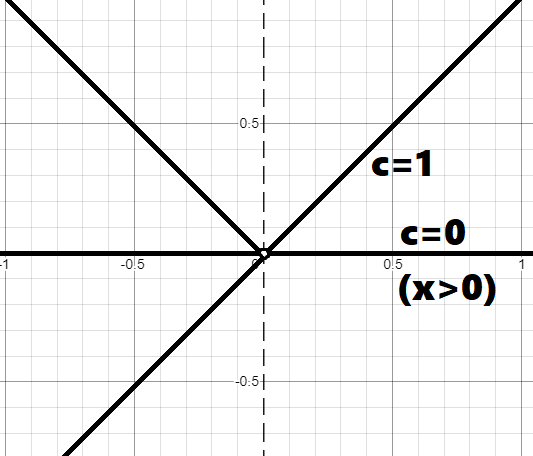
\includegraphics[scale=0.3]{pics/EasyIsoclines.png}\\
    \[x \neq 0,\q \frac{y}{x}=c(=tg \alpha)\text{ - уравнение изоклин}\]
    \[(y'=f(x,y) \Ra y'=c \Ra f(x,y)=c)\]
    \[\Ra y=cx\]
    \[\text{При } c=0\ (\ctg \alpha = 0 \Ra \alpha = 0) \Ra y=0\]
    \[\text{При } c=1\ (\ctg \alpha = 1 \Ra \alpha = \frac{\pi}{4}) \Ra y=x\]
    \[\text{З. Коши для (-1,1): }y=-x,\ x<0\]
\end{Example}

\begin{Example}[больше изоклин]
    \[y'=-\frac{y}{x} \Ra -\frac{y}{x}=c \text{ - уравнение изоклин}\]
    \[\Ra c=0\ (tg \alpha = 0)\Ra y=0\]
    \[\Ra c=1\ (\alpha = \frac{\pi}{4})\Ra y=-x\]
    \[\Ra c=\sqrt{3}\ (\alpha=\frac{\pi}{3})\Ra y=-\sqrt{3}x\]
\end{Example}

\begin{Example}[16, дополнительно] \ \\
    Написать уравнение геометрического места точек перегиба графиков решений уравнений:
    \[a)\q y'=y-x^2\]
    \[b)\q y'=f(x,y)\]
\end{Example}

\begin{sol}
    Условие перегиьа графика $y=f(x)$ - это $y''=0$\\
    a) $y'=y-x^2$
    \[y''=y'-2x=(y-x^2)-2x=0 \Ra y=x^2+2x\]
    b) Возьмем полный лифференциал от обеих частей равенства:
    \[d y'=d f(x,y) \Ra
    d y'=\dfrac{\d f}{\d x}d x+\dfrac{\d f}{\d y} d y
    \Ra \dfrac{d y'}{d x} = \dfrac{\d f}{\d x}+\dfrac{\d f d y}{\d y d x}\]
    \[\Ra y''=f'_x+f'_y y'=0 \Ra f'_x+f'_y y'=0\]
\end{sol}

\begin{Example}[замена переменной спасёт]
    \[y'=\sqrt{4x+2y-1}\]
\end{Example}
    \[\text{Пусть } z=4x+2y-1 \Ra z'=4+2y' \Ra \frac{z'-4}{2}=\sqrt{z}\]
    \[\frac{z'}{2}=\sqrt{z}+2 \Ra \frac{dz}{\sqrt{z}+2}=2dx\]
    (дорешать)

\begin{Example}[не пугаться замен]
    \[y'=\cos(y-x)\]
    \[y-x=z \Ra z'=y'-1\]
    \[z'=\cos z-1\]
    \[\frac{dz}{\cos z - 1}=dx\]
    \[\cos z=1\]
    \[z=2\pi k,\q k \in \Z\]
    \[y=x+2\pi k\]
\end{Example}

\begin{Example}[асимптота]
    \[y'=y^2-1,\q y \equiv 1,\ y \equiv -1\]
    \[y'>0 \lra y^2>1\]
    \[y'<0 \lra y^2<1\]
    \[y''=2y y'\]
    \[y''=2yy(y^2-1)\]
    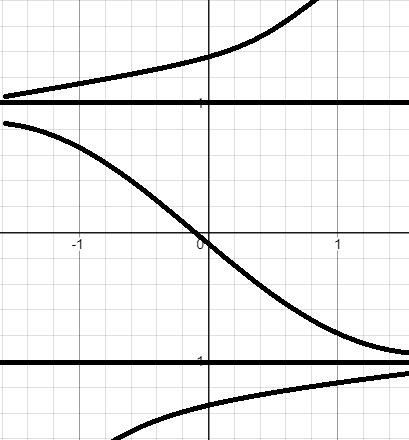
\includegraphics[scale=0.3]{pics/resh1.png}
\end{Example}

\begin{example}[теоретическая задача]
    Доказатать, что решение ограничено сверху или снизу\\
    \[Y'=P_n(y),\ n=2m-1,\ m \in \N\]
    У многочлена нечетной степени всегда есть вещественный корень, $y_j$ - корень, $j=1,...,k$, $y=y_j$ - реш. Значит остальные решения не пересекают на графике это $\Ra$ те котороые снизу, ограничены сверху, те которые сверху ограничены снизу\\
    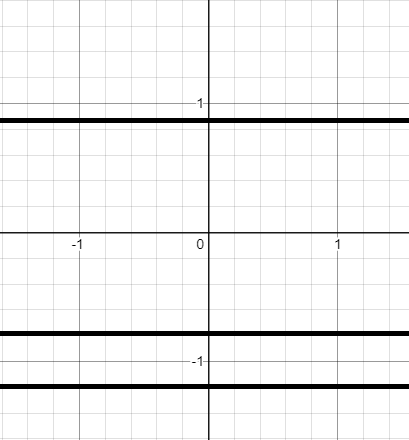
\includegraphics[scale=0.3]{pics/resh2.png}
\end{example}

\begin{example}[24, дополнительно]
  Составить диф. уравнение для семейства линий $y=a x^2 + b e^x$
  \[\Ra
  \begin{cases}
    y'=2a x + b e^x\\
    y'=2a + b e^x
  \end{cases}\]
  Нетрудно найти:
  \[a=\frac{y'-y''}{2(x-1)}\]
  Подставляя во второе уравнение:
  \[b=\frac{y'' x - y'}{e^x (x-1)}\]
  После подстановки в исходное:
  \[y'' x(x-2)-y'(x^2-2)+2(x-1)y=0\]
\end{example}

\section{Геометрические уравнения}

\begin{Example}
    \[y'=\frac{y}{x+y}\]
    \[y \neq x\]
    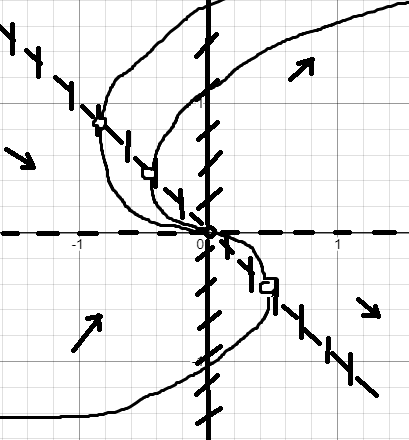
\includegraphics[scale=0.3]{pics/resh3.png}\\
    \[y \equiv 0\text{ - реш}\]
    \[y+x>0 \equiv y>-x\]
    \[y>0\]
    \[\frac{y}{z+y}=c \text{ - ур-ие изоклин}\]
    \[c=1 \q y=x+y\]
    \[y=cx+cy\]
    \[y(1-c)=cx\]
    \[y=\frac{c}{1-c}x,\q c \neq 1\]
    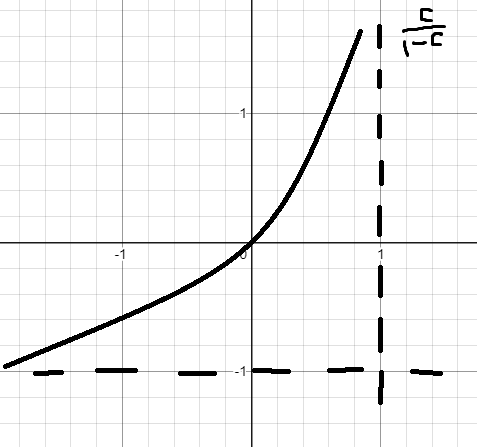
\includegraphics[scale=0.3]{pics/resh4.png}\\
    (упр.) Подставить точки
\end{Example}

\begin{example}
    \[y'=y-x^2 \Ra y=x^2+c\]
    Сократится тогда, когда уравнение второй степени $y=x^2+ax+b$, подставим: $2x+a=ax+b \Ra a=2 \ b=2$, значит $y=x^2+2x+2$ - решение\\
    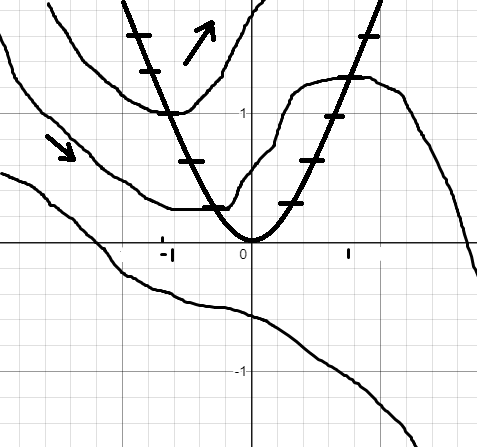
\includegraphics[scale=0.3]{pics/resh5.png}
    \[y''=y'-2x=y-x^2-2x,\q y=x^2+2x\]
\end{example}

\begin{example}\ \\
    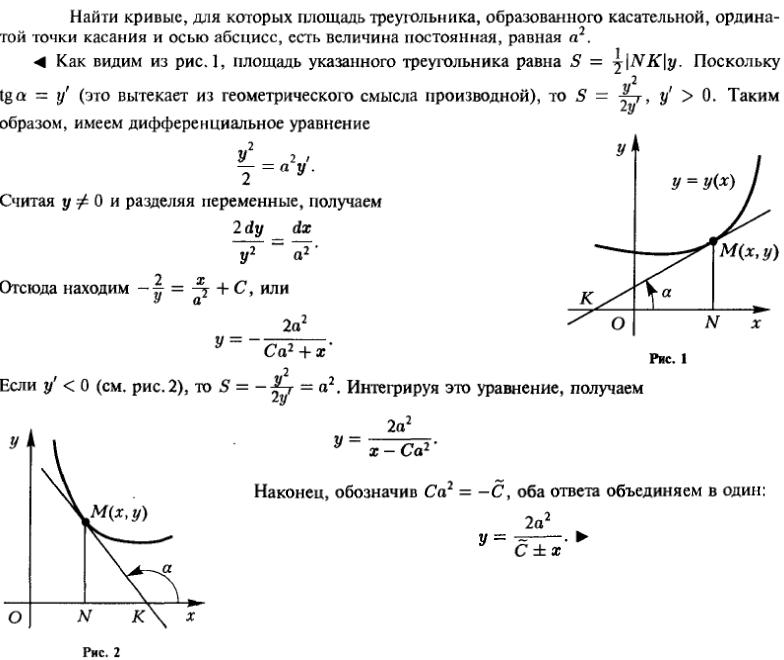
\includegraphics[scale=0.7]{pics/z71.jpg}
\end{example}

\section{Однородные уравнения}
\begin{definition}
    $M(x,y)$ - однор. ур-ие степени k, если $\forall \lambda>0$ $M(\lambda x, \lambda y) \lambda^k M(x,y)$
\end{definition}

\begin{definition}
    Уравнение $M(x,y) dx + N(x,y) dy=0$ - однородное, если $M,N$ - однородное одинаковой степени k
\end{definition}

\begin{definition}
    Уравнение $y'=f(x,y)$ - однородное, если $f(x,y)$ - однородное степени 0
\end{definition}

\begin{example}[однородное уравнение]
    $x y'-y=x \tg \frac{y}{x}$\\
    $y'=\frac{y}{x}+\tg \frac{y}{x}$\\
    Замена $y=t x$\\
    То есть мы подставляем сперва $y=ay$, $x=ax$ и если a сокращаются, то уравнение однородное и можно сделать замену $y=tx$\\
    $y'=t' x+t$\\
    $dy=t dx+x dt$\\
    $t' x = \tg t$
\end{example}
\\
Дз: 73, 76, 80, 84, 107, 109, 110, 101-112 (выбрать любую), 113

\begin{example}[пересекающиеся прямые]
    $(2x-4+6)dx+(x+y-3)dy=0$, чтобы сделать его однородным сделаем замену из системы (они не 0)\\
    $\begin{cases} 2x-4+6 = 0 \\ x+y-3=0 \end{cases} \Ra \begin{cases} x=\w{x}+1 \\ y=\w{y}+2 \end{cases}$\\
    $(2\w{x}-4\w{y})d\w{x}+(\w{x}+\w{y})d{y}=0$\\
    $\w{y}=t\w{x} \Ra d\w{y}=\w{x}dt+td\w{x}$\\
    И так далее
\end{example}

\begin{Example}[параллельные прямые]
    \[(2x+y+1)dx+(4x+2y-3)dy=0\]
    \[2x+y+1=z \Ra 4x+2y-3=2z-5\]
    \[2dx+dy=dz \Ra dy=dz-2dx\]
    \[z dx-(2z-5)(dz-2dx)=0\]
    Решаем уравнение для $\dfrac{dz}{dx}$ и возващаемся к прежним переменным
\end{Example}

\begin{example}[страшное выражение]
    $2x dy+(\underbrace{x^2 y^4} + \underbrace{1})y dx=0$\\
    Степени должны быть равны при замене $y=z^m$, если это однородное, то есть $2+4m=0 \Ra m=-\frac{1}{2}$\\
    $y=\frac{1}{\sqrt{z}}$, если y>0\\
    $y=-\frac{1}{\sqrt{z}}$, если y<0\\
    Но при такой замене теряем решение $y \equiv 0$\\
    При замене $y_0$ на $-y_0$ получается то же самое\\
    $x=\frac{t}{y^2} \Ra \dx=\frac{y^2 dt-2y t dy}{y^4}$\\
    $\Ra 2t dy+(t^2+1)(y dt-2t dy)=0$\\
\end{example}

ДЗ: 119, 120, 124, 127, 131, 132, 135 (любой из а-в)

\begin{Theorem}
    \[y'=p(x)y+q(x) \q p(x),q(x) \in C(a,b)\]
    \[\Ra \e ! \text{ реш. з. Коши } (x_0,y_0): x_0 \in (a,b) \q y_0 \in \R\]
\end{Theorem}
\begin{remark}
    \begin{enumerate}
    \item $y'=p(x)y+q(x)$ - лин. неоднородное $(q(x) \not \equiv 0)$
    \item $y'=p(x)y$ - лин. однородное
    \end{enumerate}
    \ \\
    Если $y_1,y_2$ - реш (2), $y_{1,2} \not \equiv 0 \Ra \e c=\const: y_2=c y_1$
\end{remark}

\begin{Proof}
    \[y_1'=p(x) y_1\]
    \[y_2'=p(x) y_2\]
    \[(\dfrac{y_2}{y_1})'=\dfrac{y_2' y_1-y_1'y_2}{y_1^2}=\dfrac{p y_2-p y_2}{y_1}=0\]
    Действительно, $y_1,y_2$ отличаются на константу\\
    Решение однор. $y=c y_1$ $\forall$частн. решение $y_1 \neq \equiv 0$
\end{Proof}

ЗДЕСЬ ЧТО-ТО ПРОПУЩЕНО, Я ОТВЛЕКСЯ НА ОБДУМЫВАНИЕ ПРОШЛОГО ДОК-ВА
\\
\section{Метод вариации произвольной переменной}
1) Решаем однородное\\
2) Варьируем const\\
Найдем общеее решение л.о.у.:
\[\RNumb{1})\q \dfrac{dy}{y}=p(x)dx\]
\[\ln|y|=\int p(x) dx+\ln|c|\]
\[y=c e^{\int p(x) dx}\]
\[\RNumb{2})\q  c'e^{\int p(x) dx}+c e^{\int p(x) dx} p(x) = p(x) c e^{\int p(x) dx} + q(x)\]
\[x'=q(x) e^{-\int p(x) dx} \Ra c(x)=\int q(x) e^{-\int p(x) dx} dx + \w{c}\]
\[y=e^{\int p(x) dx} (\int q(x) e^{-\int p(x) dx} dx+\w{c})\]
\[\text{З. К. }(x_0,y_0) \q y = e^{\int_{x_0}^x p(\tau) d\tau} (y_0+\int_{x_0}^x q(\tau) e^{-\int_{x_0}^\tau p(s) ds}d\tau)\]

\begin{Example}
    \[(2x+1)y'=4x+2y\]
    $\RNumb{1})$ Решим сперва такое уравнение: $(2x+1)y'=2y$
    \[\dfrac{dy}{y}=\dfrac{2 dx}{2x+1} \Ra \ln|y|=\ln|x+1|+\ln|c|\]
    \[y=c(2x+1)\]
    $\RNumb{2})$ $(2x+1)(2c+(2x+1)c')=4x+2c(2x+1)$
    \[c'\dfrac{4x}{(2x+1)^2}\]
    \[c=\int \dfrac{4x}{(2x+1)^2} dx=/u=2x+1/=\int \dfrac{u-1}{u^2} du =\]
    \[=\int (\dfrac{1}{u}-\dfrac{1}{u^2}) du=\ln|u|+\dfrac{1}{u}+\w{c}=\ln|2x+1|+\dfrac{1}{2x+1}+\w{c}\]
    Ответ: $y=(\ln|2x+1|+\dfrac{1}{2x+1}+\w{c})(2x+1)$
    \[\underbrace{y}_{\text{общее н.}}=\underbrace{(2x+1)\ln|2x+1|+1}_{\text{частное н.}}+\underbrace{\w{c}(2x+1)}_{\text{общее о.}}\]
\end{Example}

\begin{Theorem}[Бернулли]
    \[y'=p(x)y+q(x) y^\alpha \q \alpha \neq 0, \q \alpha \neq 1\]
    \[\alpha>0 \Ra \text{особое реш. } y \equiv 0\]
    Варьируем константу! Не делаем как в Филиппове
\end{Theorem}

\begin{Example}
    \[y'+2y=y^2 e^x\]
    \[y'=-2y \Ra y=c e^{-2x} \text{ - подставим}\]
    \[c'=c^2 e^{-x} \text{ - нужно разделить переменные}\]
    \[\int \dfrac{dc}{c^2}= \int e^{-x} dx \Ra \dfrac{1}{c}=e^{-x}+\w{c} \Ra c=\dfrac{1}{e^{-x}+\w{c}}\]
    Ответ: $y=\dfrac{1}{e^{-x}+\w{e}} e^{-2x},\q y \equiv 0$
\end{Example}

ДЗ: 136-160 (найти интересные), 146/148, 161-164, 178, 173/174

\begin{Example}[162]
    \[(x+1)(y y'-1)=y^2\]
    \[y^2=z \Ra 2y y'=z'\]
    \[(x+1)(\dfrac{z'}{z}-1)=z\]
\end{Example}

\begin{example}[174, геометрическая задача]
  Найти кривые, у которых площадь треугольника, ограниченного касательной, осью абсцисс и отрезком от начала координат до точки касания, есть величина постоянная, равная $a^2$
  \begin{figure}[H]
	    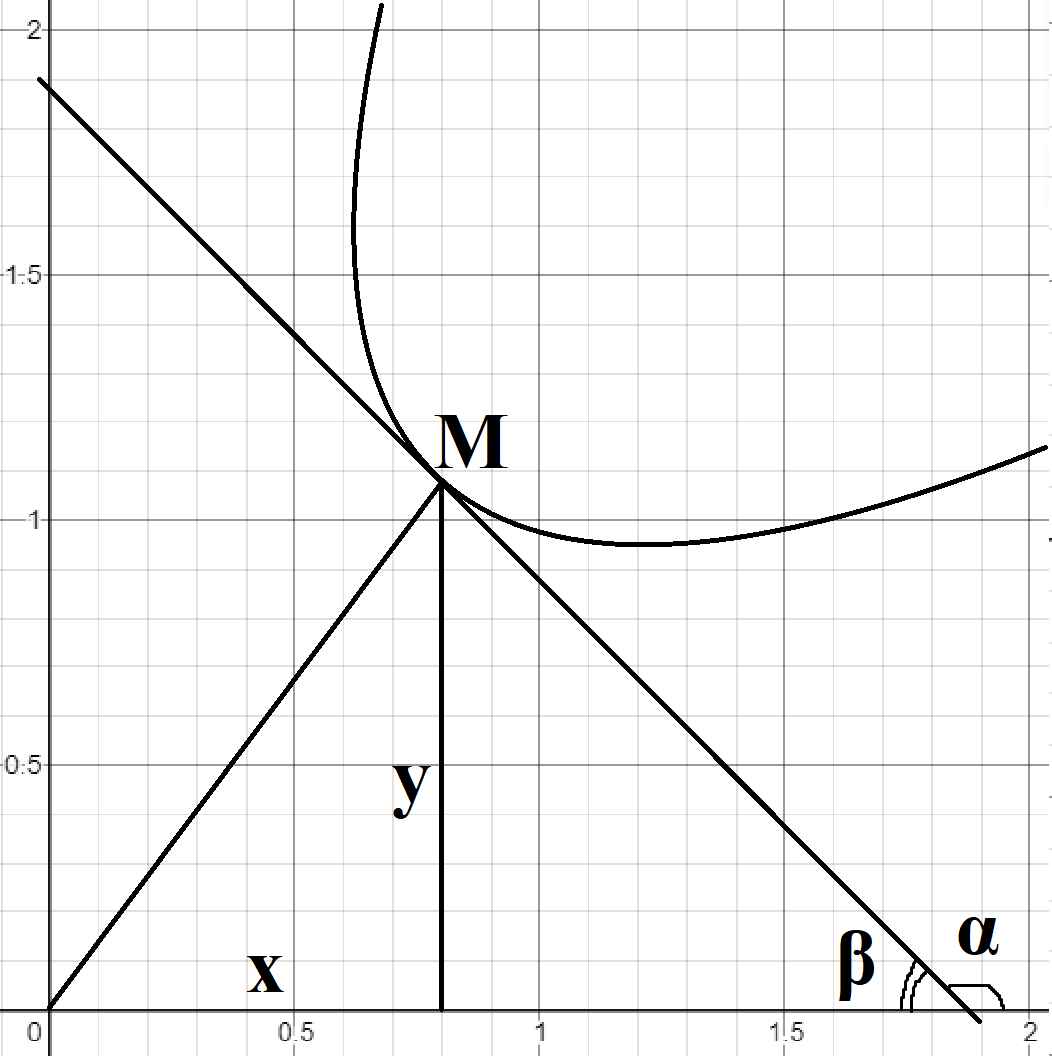
\includegraphics[scale=0.2]{pics/resh6.png}
	    \centering
	\end{figure}
  \[\tg \beta = - \tg \alpha = -y'\]
  \[\frac{1}{2} (x-\frac{y}{y'})y=a^2\]
  \[x y - 2a^2 = y^2 \frac{dx}{dy}\]
\end{example}

\begin{example}[178, мат. анализ наносит ответный удар]
  Найти то решение дифференциального уравнения
  \[y' sin 2x = 2(y + cos x),\]
  которое остается ограниченным при $x \ra \frac{\pi}{2}$\\
\end{example}

\begin{Sol}
  \[y=C\tg x+\frac{1}{\cos x}\]
  Следует, что
\end{Sol}

\begin{remark}[Риккати]
  \[y'=a(x)y^2+b(x)y+c(x) \q (1)\]
  В общем случае не интегрируется в квадратурах.
  \[y=y_1(x) \text{ - реш (1) $\Ra$ замена }y=z+y_1\]
  \[z'+y_1'=a(z^2+2zy_1+y_1^2)+b(z+y_1)+c\]
  \[z'+\cancel{y_1'}=a(z^2+2zy_1+y_1^2)+bz+\cancel{ay_1^2+by_1}+c\]
  \[z'=(2ay_1+b)z+az^2\text{ - уравнение Бернулли}\]
\end{remark}

\begin{example}
  Как подбирать? $y'+y^2=x^2+2$\\
  Попробуем подобрать степень x для y: $a^2 x^{2n}+...=x^2-2x$
  \[a=1,\q n=1\]
  \[y=x+c,\q -1+x^2+2xc+c^2=x^2-2x\Ra c=1\]
  \[y=x-1 \Ra -1+x^2-2x+1=x^2-2x\]
\end{example}

\begin{Example}[ещё пример]
  \[y'+2y^2=\frac{6}{x^2}\]
  \[y=\frac{a}{x} \Ra -\frac{a}{x^2}+\frac{2a^2}{x^2}=\frac{6}{x^2}\]
  \[2a^2-a-6=0 \Ra a=2\]
\end{Example}

\begin{Example}[171]
  \[y'+2y e^x - y^2 = e^{2x}+e^x\]
  \[y=e^x+z \Ra z'=z^2 \Ra \frac{dz}{dx}=z^2 \os{z \neq 0}{\Ra} z=-\frac{1}{x+C}\]
  Но при $z=0$ полуаем решение $y=e^x$\\
  Ответ: $y=e^x-\frac{1}{x+C},\q y=e^x$
\end{Example}

\subsection{Уравнения в полных дифференциалах. Интегрирующий множитель}
\begin{Definition}
  \[M(x,y)dx+N(x,y)dy=0 \text{ - уравнение в полных дифф, если } M,N \in C^1(G)\]
  \[\e u(x,y): du= \ub{\frac{\d u}{\d x}=u'_x}{M} dx + \ub{\frac{\d u}{\d y}=u'_y}{N} dy\]
  \[\frac{\d M}{\d y}=u''_{x y}=u''_{y x}=\frac{\d N}{\d x}\]
\end{Definition}

\begin{example}[187]
  Проверить, что данное уравнение является уравнением в полных дифференциалах, и решить его:
  \[\ub{M}{(2 - 9x y^2)x} dx + \ub{N}{(4y^2 - 6x^3)y} dy = 0\]
  \[M'_y=-18x^2 y \qq N'_x=-19 x^2 y\]
  \[M=u'_x \Ra u = \int (2x-9x^2 y^2) dx +\varphi(y)=x^2-3x^2 y^2 + \varphi(y)\]
  \[u'_y=-6x^3 y + \varphi'(y)=N=4y^3-6x^3 y\]
  \[\varphi'(y)=4y^3 \Ra \varphi(y)=y^4\]
  \[u(x,y)=x^2-3x^3 y^2 + y^4\]
  Ответ: $x^2-3x^3 y^2 +y^4 = c$,\q т.к.$du = 0 \Ra u=c$
\end{example}

Для сравнения:
\[\ub{d(x^2)}{2x dx} - \ub{\displaymode -3(y^2 \ub{d(yx^3)}{3x^2 dx} + x^3 \ub{d(y^2)}{2y dy})}{9x^2 y^2 dx - 6x^3 y dy} + \ub{d(y^4)}{4 y^3 dy}  = 0\]
Дифференциал произведения $d(x^3 y^2)$

\begin{example}[193]
  Проверить, что данное уравнение является уравнением в полных дифференциалах, и решить его:
  \[\ub{d(x^3)}{3x^2 dx}(1 + \ln y) = \ub{-d(y^2)}{2y dy} - x^3 \ub{d(\ln y)}{\frac{1}{y}dy}\]
\end{example}

\begin{Definition}
  \[M(x,y)dx+N(x,y)dy=0 \text{ - уравнение в полных дифф } (1)\]
  \[\mu=\mu(x,y) \text{ - инт. мн-ль }(1)\text{, если }(\mu M)dx+(\mu N)dy=0 \text{ - ур. в полных лиф.}\]
\end{Definition}

\begin{Example}[195, фокус]
  Решить уравнение, найдя каким-либо способом интегрирующий множитель или сделав замену переменных:
  \[(x^2 + y^2 + x)dx + y dy = 0\]
  \[(x^2+y^2)dx + \ub{\frac{1}{2}d(x^2+y^2)}{x dx+y dy} = 0\]
  \[dx+\frac{1}{2} \frac{d(x^2+y^2)}{x^2+y^2}=0\]
  Значит $\mu = \frac{1}{x^2+y^2}$
  \[dx+\frac{1}{2} d \ln (x^2+y^2)=0\]
  Ответ: $x+\frac{1}{2} \ln(x^2+y^2)=c$
\end{Example}

\begin{Example}[196, фокус]
  Решить уравнение, найдя каким-либо способом интегрирующий множитель или сделав замену переменных:
  \[(x^2 + y^2 + x)dx - x dy = 0\]
  \[(x^2+y^2)dx + y dx - x dy = 0\q d \Br{\frac{y}{x}}=\frac{dy x - y dx}{x^2}\]
  \[(1+\Br{\frac{y}{x}}^2)dx - \ub{d\Br{\frac{y}{x}}}{\frac{x dy-y dx}{x^2}}\]
  \[\mu = \frac{1}{x^2(1+\Br{\frac{y}{x}}^2)}=\frac{1}{x^2+y^2}\]
\end{Example}


ДЗ: 167-170 (интересные), 188-194 (интересные), 196, 201, 203

\section{ПРОПУЩЕННАЯ ПАРА}

\section{В ожидании кр...}

\begin{Example}
  \[xy^2(xy'+y) = 1\qq \text{Заметим, что }xy'+y = (xy)'\]
  \[xy'+y-\dfrac{1}{xy^2} = 0 \qq xy = z \Ra \dfrac{z^2}{x}z' = 1\]
  \[x dy + \dfrac{xy^3 - 1}{xy^2}dx = 0\]
  \[x^2 y^2 dy + xy^3 dx - dx = 0\]
  \[\mu = ?\]
  \[\ub{d(xy)}{x dy + y dx} - \dfrac{dx}{xy^2} = 0\]
  \[c = \dfrac{xy^3}{3} + \dfrac{x^2}{2}\]
\end{Example}

\begin{Example}[203]
  \[y(x+y)dx + (xy+1)dy = 0\]
  \[yx dx + y^2 dx + xy dy + dy = 0\]
  \[yx dx + y(\ub{d(xy)}{y dx + x dy}) + dy = 0 | \cdot \dfrac{1}{y}\]
  \[x dx + d(xy) + \dfrac{dy}{y} = 0\]
  \[\dfrac{x^2}{2} + xy + \ln |y| + c = 0\]
\end{Example}

\begin{Example}[301]
  \[xy' + x^2 + xy - y\]
\end{Example}

\begin{Proof}[похоже на частного, на однородное не тянет, но замена проходит]
  \[\dfrac{xy' - y}{x^2} + 1 \dfrac{y}{x} = 0\]
  \[y' = \dfrac{y}{x} + \dfrac{y^2}{x^2}\]
\end{Proof}

\begin{Example}[308]
  \[x^2 y' = y(x+y)\]
\end{Example}

\begin{Proof}[однородное/Бернулли]
  \[y' = \dfrac{x}{y} + \dfrac{y^2}{x^2}\]
\end{Proof}

\begin{Example}[309]
  \[(1-x^2)dy + xy dx\]
\end{Example}

\begin{Proof}[уравнение с разделяющимися переменными]

\end{Proof}

\begin{Example}[311]
  \[(y + y' \ln^2 y = (x+2\ln y)y'\]
\end{Example}

\begin{Proof}[линейное уравнение]
  \[y'_x = \dfrac{1}{x'_y}\]
  \[x'_y y = x + 2\ln y 0 \ln^2 y\]
  \[y dx - x dy (2\ln y - \ln^2 y) dy\]
\end{Proof}

\begin{Example}[320]
  \[2x^3 y y' + 3x^2 y^2 + 7 = 0\]
\end{Example}

\begin{Proof}[производная произведения]
  \[(x^3 y^2)' + 7 = 0'\]
\end{Proof}

\begin{Example}[330]
  \[(1-x^2)y^2 - 2xy^2 = xy\]
\end{Example}

\begin{Proof}[переменные разделяются, Бернелли]
  
\end{Proof}

\begin{Example}[333]
  \[(\sin x + y) dy + (y \cos x - x^2) dx = 0\]
\end{Example}

\begin{Proof}[уравнение в полных дифференциалах]
  \[\ub{d(y \din x)}{\sin x dy + y \cos x dx} - y dy - x^2 dx = 0\]
\end{Proof}

\begin{Example}[338]
  \[x(x+1)(y'-1) = y\]
\end{Example}

\begin{Example}[349]
  \[xy' = 2 \sqrt y \cos x - 2y\]
\end{Example}

\begin{Proof}[Бернулли, вариация переменной]

\end{Proof}

\begin{Example}[359]
  \[xy'(\ln y - \ln x) = y\]
\end{Example}

\begin{Proof}[однородное]
  \[y' \ln \dfrac{y}{x} = \dfrac{y}{x}\]
\end{Proof}

\begin{Example}[361]
  \[(2x^2 y - 3y^2)y' = 6x^2 - 2xy^2 +1\]
\end{Example}

\begin{Example}[368]
  \[y' = \sqrt[3]{2x - y} + 2\]
\end{Example}

\begin{Example}[371]
  \[2(x^2 y + \sqrt{1 + x^4 y^2}) dx + x^3 dy\]
\end{Example}

\begin{Example}[374]
  \[(2x+3y-1)dx + (4x + 6y - 5)dy = 0\]
\end{Example}

\begin{Proof}[параллельные прямые]
  \[2x + 3y - 1 = z \Ra 2dx + 3dy = dz\]
\end{Proof}

\begin{Example}[414]
  \[(x^2-1)y' + y^2 - 2xy + 1 = 0\]
\end{Example}

\begin{Example}[438]
  \[(2x + y + 5)y' = 3x + 6\]
\end{Example}

\begin{Proof}[пересекающиеся прямые]
  \[(2x+y+5)dy - (3x+6)dx = 0\]
  \[\text{Замена } x + 2 = \w{x}\q y + 1 = \w{y}\]
\end{Proof}
\end{document}
